%======================= PREAMBOLO DICHIARAZIONI INIZIALI===============%
\documentclass[10pt,oneside,a4paper]{article}

\usepackage[latin1]{inputenc} 
\usepackage[italian]{babel}
\usepackage{siunitx} %Inserisce automaticamente i dati con le unit�  di misura correttamente formattate del SI (utilizzo: \SI{0.82}{m^2}, in generale \SI{misura con il punto decimale}{unit�  di misura})
\sisetup{output-decimal-marker = {.}, separate-uncertainty = true, input-uncertainty-signs = \pm, detect-weight=true, detect-family=true} %per usare SI con il punto decimale
\usepackage{listings} %Per citare codice informatico formattandolo correttamente
\usepackage{amsmath}
\usepackage{graphicx}
\usepackage{geometry}
\usepackage{epigraph}
\usepackage{booktabs}	%tabelle migliorate
\usepackage{tablefootnote}	%note a pi� di pagina in tabella
\usepackage{threeparttable} %tabella con note a pi� di tabella
\usepackage{caption}	%descrizione per figure
\captionsetup{tableposition=top,figureposition=bottom,font=small} %setup descrizione
\usepackage{float}
\usepackage{esvect} %vettori
\usepackage{longtable} %tabelle lunghe
\usepackage[dvipsnames]{xcolor}
\definecolor{sepia}{HTML}{80002A}
\usepackage[colorlinks=true, citecolor=black, linkcolor=sepia, urlcolor=black]{hyperref}
\usepackage{mathrsfs}
%\usepackage[utf8]{inputenc}

\newcommand{\var}{\operatorname{var}}
\newcommand{\cov}{\operatorname{cov}}


\usepackage{listings} %Per inserire codice
\lstnewenvironment{codice_c}[1][]
{\lstset{basicstyle=\small\ttfamily, columns=fullflexible,
keywordstyle=\color{red}\bfseries, commentstyle=\color{blue},
language=C, basicstyle=\small,
numbers=left, numberstyle=\tiny,
stepnumber=2, numbersep=5pt, frame=shadowbox, #1}}{}

\setcounter{section}{-1}

%========= PRIMA PAGINA ===========%
\title{\textsc{Studio del moto di un volano}}
\author{\small{G. Galbato Muscio} \and \small{L. Gravina} \and \small{L. Graziotto} \and \small{M. Rescigno}}
\date{}

\begin{document}
	\begin{figure}
		\centering
		
\includegraphics[scale=0.5, trim={2.8cm 8.9cm 0 9cm}, clip]{logo.png}
	\end{figure}
	\maketitle
	\begin{center} 
		\fbox{{\fontsize{12pt}{8mm}\textsc{Gruppo B2.3}}} \\
		\vspace{1cm}
		\begin{tabular}{ccc}
			Esperienza di laboratorio && Consegna della relazione \\
			\emph{\small{24 maggio 2017}} && \emph{\small{30 maggio 2017}} \\
		\end{tabular} 
		
		\vspace{0.5cm}
		
	\end{center}
\hrule
\vspace{0.5cm}
\begin{abstract}
Si studiano le leggi orarie che descrivono il moto di un volano, e da queste si misurano il momento d'inerzia del volano e il momento frenante che ne ostacola la rotazione, anche dipendente dall'attrito con l'aria.
\end{abstract}
\newpage
\tableofcontents %Indice
\listoftables %Indice delle tabelle
\listoffigures %Indice dei grafici
\pagebreak
\section{Convenzioni e formule}
In questa relazione verranno usate le seguenti convenzioni:
\begin{enumerate}
	\item sar� usato il punto [ $.$ ] come separatore decimale;
	\item l'approssimazione decimale della cifra $5$ sar� fatta per eccesso;
	\item al fine di snellire la relazione e migliorarne la leggibilit�, riporteremo nel corpo del documento solamente le tabelle riepilogative e alcuni grafici, e dedicheremo un'appendice finale alle tabelle e ai grafici pi� dettagliati.
\end{enumerate}
Inoltre, si far� riferimento alle seguenti formule:
\begin{enumerate}
	\item media 
	\begin{equation}\label{eq:media}
	\bar{x} = \frac{1}{N}\sum_{i=1}^Nx_i;
	\end{equation}
	\item varianza
	\begin{equation}\label{eq:varianza}
	\sigma^2 = \frac{1}{N}\sum_{i=1}^N(x_i-\bar{x})^2;
	\end{equation}
	\item deviazione standard
	\begin{equation}\label{eq:deviazione}
	\sigma = \sqrt{\sigma^2}.
	\end{equation}	
\end{enumerate}
Per ricavare i parametri della regressione lineare si utilizzeranno le seguenti equazioni: 
\begin{enumerate}
	\item coefficiente angolare
	\begin{equation}\label{eq:coefficienteangolare}
	\hat{m} = \frac{\overline{xy}-\bar{x}\bar{y}}{\overline{x^2}\bar{x}^2};
	\end{equation}
	\item intercetta
	\begin{equation}\label{eq:intercetta}
	\hat{c} = \bar{y} - \hat{m} \cdot \bar{x};
	\end{equation}
	\item varianza del coefficiente angolare
	\begin{equation}\label{eq:varianzacoeff}
	\var[\hat{m}] = \frac{1}{\var[x]\cdot \sum_{i}\frac{1}{\sigma_{y_i}^2}};
	\end{equation}
	\item varianza dell'intercetta 
	\begin{equation}\label{eq:varianzainter}
	\var[\hat{c}] = \bar{x^2}\cdot \var[\hat{m}];
	\end{equation}
	\item covarianza 
	\begin{equation}\label{eq:cov}
	\cov[\hat{m}, \hat{c}] = - \frac{\bar{x}}{\var[\hat{m}]\cdot \sum_{i}\frac{1}{\sigma_{y_i}^2}}.
	\end{equation}
\end{enumerate}

%===============SCOPO E DESCRIZIONE DELL'ESPERIENZA==============%
\section{Scopo e descrizione dell'esperienza}
\label{sec:descrizione}
Un volano consiste in un disco metallico di momento d'inerzia $I_0$, vincolato a ruotare attorno ad un asse fisso orizzontale passante per il suo centro. Ad esso � possibile avvitare, nei pressi del bordo, alcuni bulloni al fine di aumentarne il momento d'inerzia. Esso � collegato, mediante un filo passante per una puleggia di massa trascurabile, ad una zavorra che, scendendo, mette in moto rotatorio il disco. Considerando il filo inestensibile e di massa trascurabile si ha che l'accelerazione $a$ a cui scende la zavorra � legata all'accelerazione angolare di rotazione del volano $\alpha$ dalla relazione $a = \alpha r$, dove $r$ � il raggio del disco pi� piccolo, collegato al volano, attorno al quale si avvolge il filo (si veda la figura~\ref{fig:schema_apparato}). Il disco � soggetto ad un momento frenante $M_a$ dovuto agli attriti dell'asse di rotazione con la sede entro la quale ruota; inoltre, al volano possono essere applicate delle palette al fine di incrementare l'attrito con l'aria e studiare la velocit� limite $v_\text{lim}$ di caduta della zavorra. Nel corso dell'esperienza si daranno le stime di $I_0$, $M_a$ e del coefficiente di attrito viscoso con l'aria $k$.



%================APPARATO SPERIMENTALE======================%		
\section{Apparato Sperimentale}
\subsection{Strumenti}
\label{subsec:strumenti}
\begin{itemize}
	\item Sensore di posizione che misura la posizione della massa $m$ a tempi diversi;
	\item Metro [divisione: \SI{0.001}{m}, incertezza: \SI{0.0003}{m}];
	\item Calibro ventesimale [divisione \SI{0,05}{mm}, incertezza \SI{0,05}{mm}, portata \SI{20}{cm}];
	\item Bilancia di precisione [portata: \SI{2000}{g}, incertezza: \SI{0.03}{g}];
\end{itemize}
\subsection{Campioni}
\begin{itemize}
	\item Volano; 
	\item $10$ coppie di bulloni da inserire sul disco del volano; 
	\item $2$ palette per aumentare l'attrito del mezzo.
\end{itemize}

%==================SEQUENZA OPERAZIONI SPERIMENTALI==========
\section{Sequenza Operazioni Sperimentali} 

\subsection{Estrazione del momento della forza d'attrito e del momento d'inerzia}

Inserendo due coppie di bulloni per misura, senza compromettere la simmetria del sistema analizzato, studiamo il moto di discesa della massa $m$. Prima di cominciare l'acquisizione si verifica la linearit� e la correttezza della misura di posizione del sensore, verificando la lunghezza in alcuni punti con il metro. Per ogni coppia di bulloni sono state acquisite $10$ misure di velocit� in funzione del tempo. Le diverse stime dell'accelerazione sono ottenute dal coefficiente angolare delle rette che interpolano tali velocit�. Ognuna delle misure di accelerazione cos� ottenute � affetta da un'incertezza fornitaci dal programma \emph{DataStudio\textsuperscript\textregistered}. Poich� queste incertezze sono disomogenee, per tenerne conto calcoliamo la media pesata dell'accelerazione per ogni raccolta. I dati sono riportati nella tabella~\ref{tab:accvsbulloni} con le rispettive incertezze, ottenute sommando in quadratura l'incertezza da associare alla media pesata (per definizione $1/\sqrt{\sum_{i}p_i}$, con $p_i = 1 / \sigma_{a_i}^2$) e la deviazione standard della media ($\sigma/\sqrt{10}$).
Poich� l'inverso dell'accelerazione e il numero di bulloni inseriti sono legati da una relazione lineare � possibile ottenere una stima del momento d'inerzia del disco del volano, $I_0$, e del momento dell'attrito radente, $M_a$. Partendo dalle equazioni cardinali della dinamica otteniamo: 
	
	\begin{equation}\label{eq:equazioneretta}
	\frac{1}{a}= A + B\cdot n
	\end{equation}
	
dove $n$ � il numero di coppie di bulloni, mente \emph{$A$} e \emph{$B$} sono rispettivamente :
	
	\begin{equation}\label{eq:intercettaecoefficente}
	A = \frac{mr^2+I_0}{mgr^2-M_a r}; \qquad B = \frac{2m_b R^2}{mgr^2-M_a r}.
	\end{equation}

Una volta stimati, utilizzando il metodo dei minimi quadrati, l'intercetta ($A$) e il coefficiente angolare ($B$) della retta che meglio approssima i punti sperimentali, ricaviamo:

\begin{equation}\label{eq:momentoattrito}
M_a = mgr - \frac{2m_b R^2}{Br}
\end{equation}

\begin{equation}\label{eq:momentoinerzia}
I_0 = 2m_bR^2 \frac{A}{B} - mr^2
\end{equation}

Dove si ha:
\begin{itemize}
	\item $m$ = \SI{555.00 \pm 0.03 e-3}{kg}: massa appesa al filo inestensibile del volano; 
	\item $m_b$ = \SI{53.6 \pm 0.2 e-3}{kg}: media delle masse dei $16$ bulloni; 
	\item $r$ = \SI{1.068 \pm 0.009 e-2}{m}: raggio del dischetto attaccato al volano attorno al quale si avvolge il filo;
	\item $R$ = \SI{0.1753 \pm 0.0003}{m}: distanza tra l'asse di rotazione del volano e il centro di massa dei bulloni;
	\item $g$ = \SI{9.803}{m/s^2}: accelerazione di gravit�, data, in questo caso, senza incertezza. 
\end{itemize}


Gli errori da associare alla stima di $M_a$ e $I_0$ sono dati dalla propagazione delle incertezze. Derivando parzialmente rispetto ai parametri delle equazioni~\ref{eq:momentoattrito} e~\ref{eq:momentoinerzia} otteniamo:

\begin{equation}\label{eq:incertezzamomentoattrito}
\sigma_{M_a}^2= \frac {\partial{M_a}}{ \partial m} ^2 \cdot \sigma_m^2 + \frac {\partial{M_a}}{ \partial r} ^2 \cdot \sigma_r^2 + \frac {\partial{M_a}}{ \partial R} ^2 \cdot \sigma_R^2 + \frac {\partial{M_a}}{ \partial m_b} ^2 \cdot \sigma_{m_b}^2 + \frac {\partial{M_a}}{ \partial B} ^2 \cdot \sigma_{B}^2 
\end{equation}

Dove con $\sigma_m$, $\sigma_R$ e $\sigma_r$ intendiamo l'incertezza sulla massa, sulla distanza tra asse di rotazione e bulloni e sul raggio del dischetto date dalle rispettive incertezze strumentali, e con $\sigma_{m_b}$ l'incertezza sul valor medio della massa dei bulloni, data dalla somma in quadratura dell'incertezza strumentale e statistica (deviazione standard della media). Con $\sigma_B$ indichiamo invece l'errore sul coefficiente angolare stimato con il metodo dei minimi quadrati (in particolare � la radice della varianza calcolata con~\ref{eq:varianzacoeff}).

Derivando parzialmente si ottiene dalla~\ref{eq:incertezzamomentoattrito}:
\small{
\begin{equation}
\sigma_{M_a}^2= (gr)^2 \cdot \sigma_m^2 + \left(mg + \frac{2m_b R^2}{Br^2}\right) ^2 \cdot \sigma_r^2 + \left(-\frac{4m_bR}{Br}\right)^2 \cdot \sigma_R^2 + \left(-\frac{2R^2}{Br}\right)^2 \cdot \sigma_{m_b}^2 + \left(\frac{2m_b R^2}{B^2 r}\right)^2 \cdot \sigma_{B}^2 
\end{equation}
}

L'errore sul momento d'inerzia del volano � ottenuto con lo stesso procedimento, per cui:
\small{ 
\begin{equation}\label{eq:incertezzamomentoinerzia}
\sigma_{I_0}^2 = \frac {\partial{I_0}}{ \partial m} ^2 \cdot \sigma_m^2 + \frac {\partial{I_0}}{ \partial r} ^2 \cdot \sigma_r^2 + \frac {\partial{I_0}}{ \partial R} ^2 \cdot \sigma_R^2 + \frac {\partial{I_0}}{ \partial m_b} ^2 \cdot \sigma_{m_b}^2+ \frac {\partial{I_0}}{\partial B} ^2 \cdot \sigma_{B}^2 + \frac {\partial{I_0}}{\partial A} ^2 \cdot \sigma_{A}^2 + 2 \frac{\partial I_0}{\partial B} \frac{\partial I_0}{\partial A} \cov(A, B)
\end{equation} 
}

Dove le incertezze sono le stesse citate precedentemente, eccetto per $\sigma_A$ che indica l'errore sull'intercetta anch'esso stimato con il metodo dei minimi quadrati (in particolare con la radice della varianza~\ref{eq:varianzainter}). Poich� i parametri $A$ e $B$ sono stati stimati a partire dallo stesso insieme di dati, si � reso necessario inserire anche il termine di covarianza. Derivando e sostituendo nella~\ref{eq:incertezzamomentoinerzia} si ottiene: 
\begin{equation}
\begin{split}
\sigma_{I_0}^2 = (-r^2)^2 \cdot \sigma_m^2 + (-2mr)^2 \cdot \sigma_r^2 + \left(4Rm_b \frac{A}{B}\right)^2 \cdot \sigma_R^2 + \left(2R^2 \frac{A}{B}\right)^2 \cdot \sigma_{m_b}^2+ \\ 
+ \left(-\frac{2m_bR^2 A}{B^2}\right)^2 \cdot \sigma_{B}^2 + \left(\frac{2m_bR^2}{B}\right)^2 \cdot \sigma_{A}^2 + 2 \left(-\frac{2m_bR^2 A}{B^2}\right) \left(\frac{2m_bR^2}{B}\right) \cov(A, B)
\end{split} 
\end{equation}


I valori dei parametri $A$ e $B$ ottenuti con le equazioni~\ref{eq:coefficienteangolare} e \ref{eq:intercetta}, a partire dai dati riportati in tabella~\ref{accvsbulloni} sono: 

\begin{equation}
\boxed{\bf{A = \SI{19.71 \pm 0.09}{s^2 / m}}};
\end{equation}
\begin{equation}
\boxed{\bf{B = \SI{5.52 \pm 0.03}{s^2 / m}}}.
\end{equation}

In figura~\ref{fig:n_vs_inva} � riportato il grafico di $1 / a$ in funzione del numero $n$ di coppie di bulloni avvitate sul volano.
%I valori di intercetta e coeficiente angolare della retta forniti dal softwer di analisi dati \emph{R} sono: 
%\begin{equation}
%B = 5.511 \qquad A = 19.750
%\end{equation}
%che risultano compatibili con le stime realtizzate manualmente di tali parametri. 

La migliore stima di $M_a$ � quindi: 
\begin{equation}
\boxed{\bf{M_a = \SI{0.0022 \pm 0.0006}{N m}}};
\end{equation}
mentre la migliore stima di $I_0$ �: 
\begin{equation}
\boxed{\bf{I_0 = \SI{0.01170 \pm 0.00012}{kg m^2}}}.
\end{equation}



\subsection{Studio della perdita di energia potenziale gravitazionale a causa del momento di attrito}

\subsection{Studio del moto del volano in presenza di attrito del mezzo}
Si montano sul volano, avvitandole con due bulloni, le due palette, di massa \SI{74.30 \pm 0.03}{g} e \SI{74.00 \pm 0.03}{g}, in posizione simmetrica. Si acquisisce la velocit� di caduta della zavorra per tre moti successivi; a titolo d'esempio la posizione della massa in funzione del tempo per uno di questi moti � rappresentata nel grafico di figura~\ref{fig:caduta_attrito_aria}, mentre la velocit� in funzione del tempo nel grafico di figura~\ref{fig:vel_attrito_aria}. Si osserva dai grafici che la zavorra raggiunge la velocit� limite dopo circa \SI{7}{s} dalla partenza, e inverte il moto al termine della caduta dopo circa \SI{23}{s} dalla partenza. Per calcolare la velocit� limite $v_\text{lim}$ si calcola dunque la media delle velocit� comprese negli intervalli di tempo in cui la zavorra scende a velocit� costante per i $3$ set di dati relativi alla caduta, e ad essa si associa un'incertezza data dalla somma in quadratura della deviazione standard divisa per la radice del numero di dati utilizzati, nel nostro caso $2646$, e dell'incertezza strumentale del sensore di posizione, che assumiamo sia pari all'ultimo digit diviso $\sqrt{12}$. Si ottiene il valore
\begin{equation}\label{eq:vlim}
v_\text{lim} = \SI{0.0665 \pm 0.0004}{m/s}
\end{equation}

Il moto della zavorra e del volano in presenza di attrito del mezzo � descritto dall'equazione differenziale
\[
\frac{d v}{d t} = \frac{1}{\tau}(v_\text{lim} - v)
\]
ove con $\tau$ si indica il tempo caratteristico,
\[
\tau = \frac{mr^2 + I_0}{kr^2};
\]
la precedente equazione ha soluzione
\[
v = v_\text{lim}(1 - e^{-t / \tau}).
\]
Con $k$ si indica il coefficiente di attrito dell'aria, che � legato alla velocit� per determinare il momento di attrito del mezzo dall'equazione di Stokes
\[
M_v = k v r,
\]
la velocit� limite � invece espressa dall'equazione
\[
v_\text{lim} = \frac{mgr^2 - M_a r}{kr^2},
\]
da cui si ricava
\[
k = \frac{mgr^2 - M_a r}{v_\text{lim}r^2}.
\]
Si ottiene perci� per il coefficiente di attrito il valore
\[
\boxed{\bf{k = \SI{79.4 \pm 0.4}{kg / s}}},
\]
con incertezza propagata

\begin{figure}
\caption{Posizione della zavorra in funzione del tempo in presenza di attrito del mezzo}
\label{fig:caduta_attrito_aria}
\centering
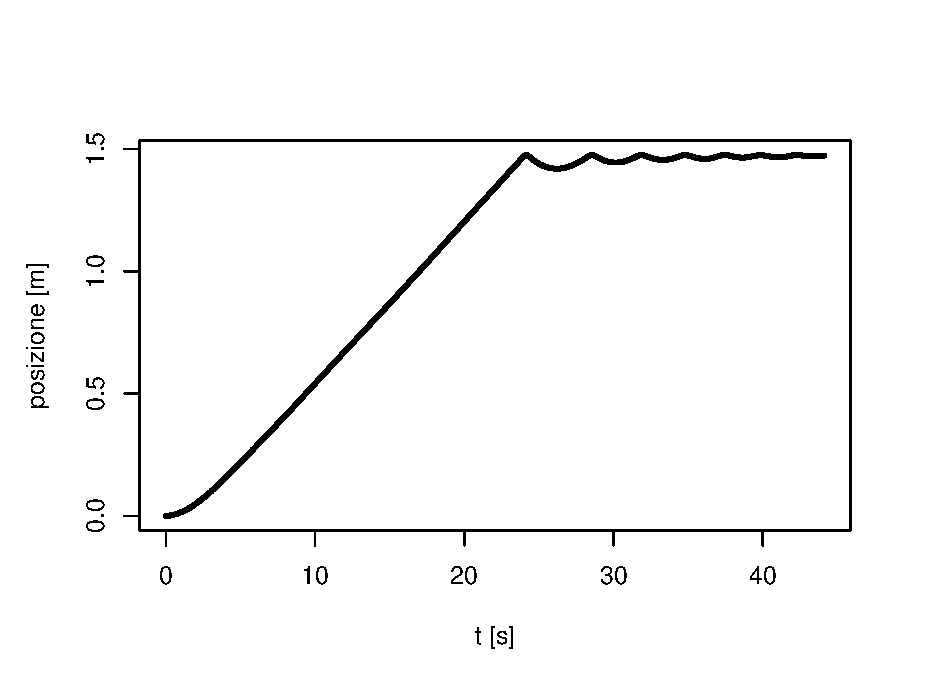
\includegraphics[scale=0.8]{caduta_attrito_aria.eps} 
\end{figure}

\begin{figure}
\caption{Velocit� della zavorra in funzione del tempo in presenza di attrito del mezzo}
\label{fig:vel_attrito_aria}
\centering
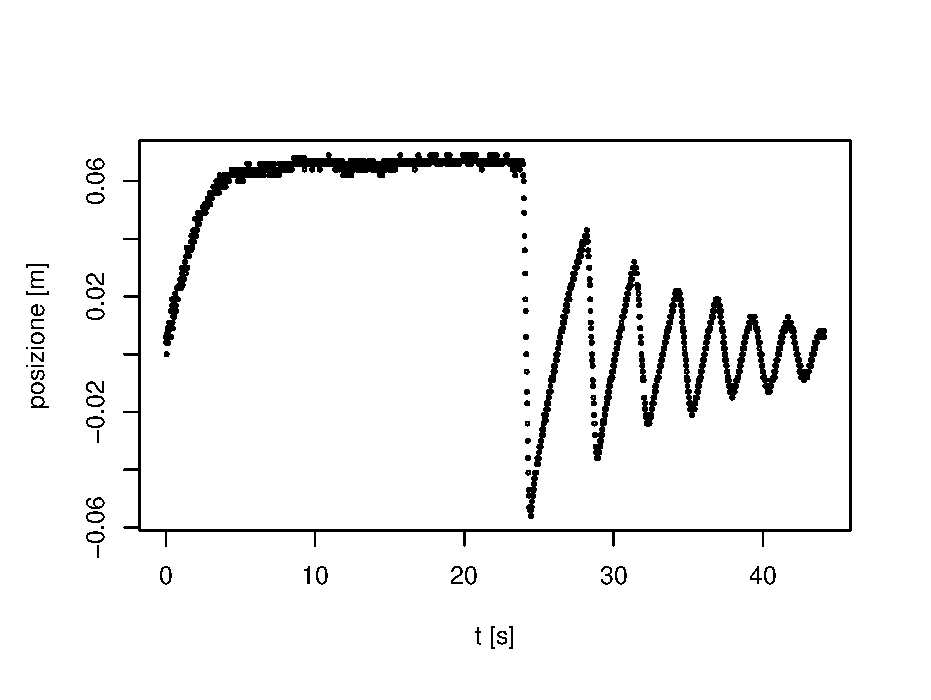
\includegraphics[scale=0.8]{vel_attrito_aria.eps} 
\end{figure}





%========================= CONCLUSIONI =============
\section{Considerazioni finali}

\pagebreak
%=================APPENDICE==================================

\section{Appendice: tabelle e grafici}


\end{document}
